\documentclass{article} 
\usepackage{polski} 
\usepackage[utf8]{inputenc} 
\usepackage[OT4]{fontenc} 
\usepackage{graphicx,color} 
\usepackage{url} 
\usepackage[pdftex,hyperfootnotes=false,pdfborder={0 0 0}]{hyperref} %za wszystkimi pakietami; pdfborder nie wszedzie tak samo zaimplementowane bo specyfikacja nieprecyzyjna; pod miktex'em po prostu nie widac wtedy ramek

\title{Automatyczna kompozycja kontrapunktu, gatunek I}
\author{Piotr Szachewicz}

\begin{document}
\maketitle

\section{Opis problemu}

Kontrapunkt jest techniką kompozytorską, która polega na prowadzeniu kilku niezależnych linii melodycznych zgodnie z określonymi zasadami harmonicznymi i rytmicznymi~\cite{wikiCounterpoint}.

W innym znaczeniu kontrapunkt oznacza melodię, która jest dokomponowywana do istniejącej już melodii, zwanej \emph{głosem głównym}, lub \emph{cantus firmus} \cite{Sikorski}.

Celem pracy jest zaprojektowanie i implementacja programu, który byłby zdolny do automatycznej kompozycji kontrapunktu (gatunek I) zgodnie z opisanymi niżej zasadami dla podanej przez użytkownika melodii \emph{cantus firmus}.

W ramach pracy ograniczono się jedynie do najprostszego rodzaju kontrapunktu, tj. do gatunku I. Przykład kontrapunktu w gatunku I przedstawiono na rysunku~\ref{fig:kontrapunkt_przyklad_gawlas}.

\begin{figure}[htb]
\centering
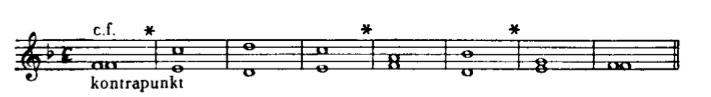
\includegraphics[width=1.0\textwidth]{images/kontrapunkt_przyklad_gawlas.png}
\caption{Przykład kontrapunktu, gatunek I. Górna linia melodyczna oznaczona skrótem \emph{c.f.} to \emph{cantus firmus}, a dolna to linia kontrapunktująca. (Źródło:~\cite{gawlas})}
\label{fig:kontrapunkt_przyklad_gawlas}
\end{figure}

W gatunku I \emph{cantus firmus} składa się z nut o jednakowych wartościach rytmicznych, a jednej nucie z głosu głównego odpowiada dokładnie jedna nuta z głosu kontrapunktującego.

Obowiązują następujące zasady harmoniczne:

\begin{itemize}
\item wszystkie współbrzmienia to konsonanse (pryma czysta, kwinta czysta, oktawa czysta, tercja mała lub wielka, seksta mała lub wielka);
\item rozpoczęcie i zakonczenie to współbrzmienie konsonansu doskonałego (pryma czysta, kwinta czysta, oktawa czysta);
\item wszystkie wertykalne konsonanse doskonałe musza być osiagniete ruchem przeciwnym (oba głosy w przeciwnych kierunkach) lub bocznych (jeden głos porusza się, a drugi jest nieruchomy).
\end{itemize}

Melodia kontrapunktu powinna spełniać następujące zasady melodyczne:

\begin{itemize}
\item przeważają kroki (ruch o sekunde małą lub wielką);
\item przeważa ruch przeciwny (oba głosy powinny poruszać się w przeciwnych kierunkach);
\item niedozwolone są skoki melodii o: tryton, septyma wielka lub mała.
\end{itemize}

Powyższe zasady są zasadami ścisłymi, które powinny obowiązywać dla każdego kontrapunktu. Poza zasadami ścisłymi wyróżnia się również zasady swobodne, które mają mniejszą wagę, np.:

\begin{itemize}
\item mieszaj konsonanse doskonałe (pryma czysta, kwinta czysta, oktawa czysta) i niedoskonałe (tercje, seksty);
\item unikaj prymy czystej w pierwszym i ostatnim współbrzmieniu;
\item unikaj skoku w obu głosach na raz;
\item po dużym skoku powinna nastąpić zmiana kierunku melodii i kroki sekundowe;
\item na przestrzeni 10-20 dźwieków głosu kontrapunktujacego z należy wykorzystać cały zakres dostępnej skali.
\end{itemize}

Dla uproszczenia problemu implementacja oparta zostanie jedynie na zasadach ścisłych.

\section{Szkic rozwiązania}

Implementacja składa się z następujących modułów:
\begin{itemize}
\item generatora,
\item funkcji oceniającej,
\item algorytmu przeszukiwania.
\end{itemize}

Moduły te zostaną omówione w poniższych podrozdziałach.

\subsection{Generator}

Celem generatora jest wygenerowanie wszystkich możliwych kontrapunktów, które będą zgodne z przedstawionymi powyżej zasadami ścisłymi dotyczącymi harmonii.
Ponadto uwzględnia on skalę dźwięków, z których może składać się kontrapunkt.

Algorytm generatora działa następująco:
\begin{enumerate}
\item Dla każdej nuty w \emph{cantus firmus} obliczane są wysokości dźwięków, które są odległe od niej o konsonse doskonałe i niedoskonałe. Dla każdej nuty \emph{głosu głównego} obliczany i przechowywany jest zbiór dozwolonych dźwięków kontrapunktu.
\item Z obliczonych zbiorów usuwane są dźwięki, które nie należą do zdefiniowanej skali.
\item Zbiór możliwych melodii, które generator jest w stanie wygenerować jest równy iloczynowi kartezjańskiemu zbiorów obliczonych w punkcie 1. (Jest to przestrzeń dozwolonych rozwiązań problemu).
\end{enumerate}

\subsection{Funkcja oceniająca}

Funkcja oceniająca przypisuje każdemu kontrapunktowi liczbę punktów. Podczas oceniania uwzględniane są jedynie zasady ścisłe dotyczące melodii -- nie jest konieczne uwzględnianie zasad dotyczących harmonii, gdyż zasady te uwzględniane są podczas pracy generatora.

Melodia analizowana jest nuta po nucie. Złamanie którejś z zasad powoduje odjęcie odpowiedniej ilości punktów (zależnej od zasady) od puli punktów danego kontrapunktu. W najlepszym przypadku, jeżeli nie zostanie złamana żadna zasada, kontrapunkt może uzyskać maksymalnie $0$ punktów.

\subsection{Algorytm przeszukiwania}

W programie zaimplementowane są dwa algorytmy przeszukiwania przeszukiwanie pełne oraz przeszukiwanie przy użyciu algorytmu genetycznego.

\subsection{Pełne przeszukiwanie}

Przeszukiwanie pełne polega na przeglądnięciu i ocenie kolejno wszystkich kontrapunktów wygenerowanych przez generator. Do zbioru końcowego, który jest pokazywany użytkownikowi, wybierany jest podzbiór kontrapunktów, który uzyskał najwyższą liczbę punktów (możliwe jest również przestawienie programu w tryb poszukiwania zbioru kontrapunktów o najgorszej liczbie punktów).

\subsection{Algorytm ewolucyjny}

Lbebebbe ~\cite{Gawlas}.


\bibliography{raport}
\bibliographystyle{plain}

\end{document}

